% Training-loss figure for the four federated nodes (OLMo-2 1B, South Asia corpus).
% Preamble requirements:   \usepackage{pgfplots}   \pgfplotsset{compat=1.16}
% Use % Training-loss figure for the four federated nodes (OLMo-2 1B, South Asia corpus).
% Preamble requirements:   \usepackage{pgfplots}   \pgfplotsset{compat=1.16}
% Use % Training-loss figure for the four federated nodes (OLMo-2 1B, South Asia corpus).
% Preamble requirements:   \usepackage{pgfplots}   \pgfplotsset{compat=1.16}
% Use % Training-loss figure for the four federated nodes (OLMo-2 1B, South Asia corpus).
% Preamble requirements:   \usepackage{pgfplots}   \pgfplotsset{compat=1.16}
% Use \input{sft_train_loss_4nodes.tex} where the figure should appear.
% (Colours are colour-blind-safe and every node also has its own marker.)
\begin{figure}[t]
  \centering
  \definecolor{nodeA}{HTML}{2A78D6}
  \definecolor{nodeB}{HTML}{EB6834}
  \definecolor{nodeC}{HTML}{1BAF7A}
  \definecolor{nodeD}{HTML}{1A1A19}
  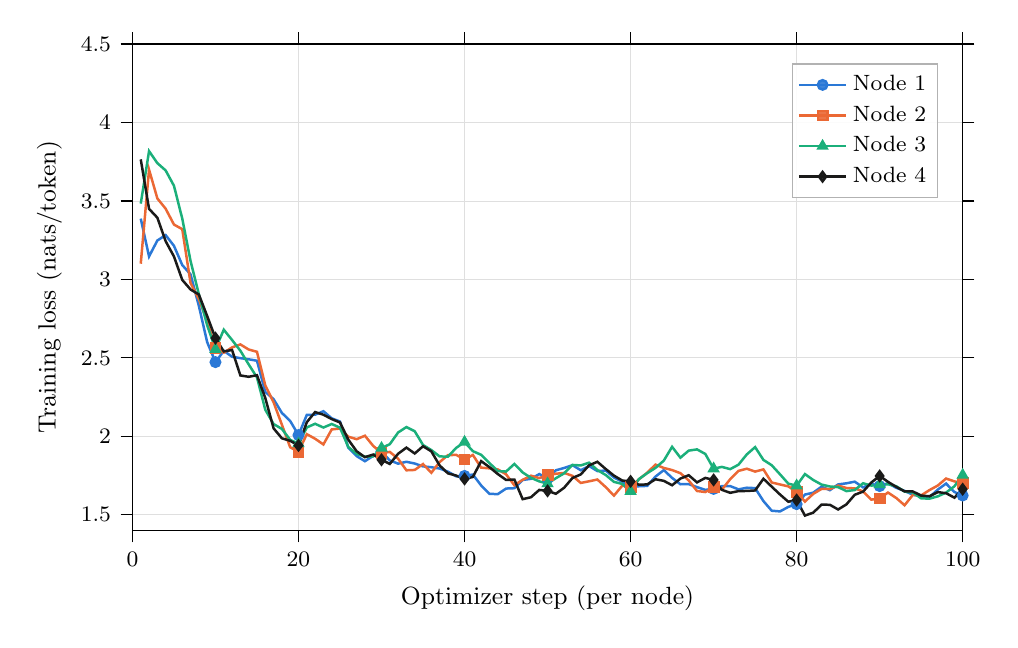
\begin{tikzpicture}
    \begin{axis}[
      width=\linewidth, height=0.64\linewidth,
      xlabel={Optimizer step (per node)},
      ylabel={Training loss (nats/token)},
      xmin=0, xmax=100, ymin=1.4, ymax=4.5,
      xtick={0,20,40,60,80,100},
      ytick={1.5,2.0,2.5,3.0,3.5,4.0,4.5},
      yticklabel style={/pgf/number format/fixed, /pgf/number format/precision=1},
      grid=major, major grid style={gray!25, line width=0.3pt},
      tick align=outside, tick style={black, line width=0.4pt},
      axis line style={black, line width=0.4pt},
      label style={font=\small}, tick label style={font=\footnotesize},
      legend style={at={(0.97,0.96)}, anchor=north east, draw=gray!60, fill=white,
                    fill opacity=0.9, text opacity=1, font=\footnotesize,
                    inner sep=2pt, /tikz/every even column/.append style={column sep=3pt}},
      legend cell align=left,
      every axis plot/.append style={line width=0.9pt, mark size=1.7pt},
    ]
    \addplot[nodeA, mark=*, mark repeat=10, mark phase=10]
      coordinates {(1,3.3874) (2,3.1464) (3,3.2481) (4,3.2825) (5,3.2141) (6,3.0918) (7,3.0323) (8,2.8312) (9,2.6006) (10,2.4731) (11,2.5449) (12,2.5076) (13,2.4983) (14,2.4912) (15,2.4819) (16,2.2834) (17,2.2370) (18,2.1494) (19,2.0980) (20,2.0082) (21,2.1366) (22,2.1382) (23,2.1602) (24,2.1150) (25,2.0943) (26,1.9274) (27,1.8743) (28,1.8417) (29,1.8757) (30,1.9024) (31,1.8468) (32,1.8261) (33,1.8380) (34,1.8270) (35,1.8087) (36,1.8034) (37,1.7951) (38,1.7752) (39,1.7453) (40,1.7481) (41,1.7566) (42,1.6875) (43,1.6338) (44,1.6320) (45,1.6675) (46,1.6697) (47,1.7222) (48,1.7295) (49,1.7596) (50,1.7327) (51,1.7840) (52,1.7986) (53,1.8166) (54,1.7843) (55,1.8112) (56,1.7789) (57,1.7822) (58,1.7378) (59,1.7114) (60,1.6760) (61,1.6821) (62,1.6844) (63,1.7437) (64,1.7851) (65,1.7354) (66,1.6949) (67,1.6958) (68,1.6765) (69,1.6591) (70,1.6652) (71,1.6827) (72,1.6832) (73,1.6622) (74,1.6728) (75,1.6702) (76,1.5877) (77,1.5263) (78,1.5218) (79,1.5506) (80,1.5680) (81,1.6290) (82,1.6413) (83,1.6793) (84,1.6573) (85,1.6939) (86,1.7009) (87,1.7113) (88,1.6749) (89,1.6978) (90,1.6833) (91,1.7020) (92,1.6721) (93,1.6526) (94,1.6281) (95,1.6190) (96,1.6125) (97,1.6607) (98,1.6993) (99,1.6458) (100,1.6232)};
    \addlegendentry{Node 1}
    \addplot[nodeB, mark=square*, mark repeat=10, mark phase=10]
      coordinates {(1,3.1001) (2,3.6995) (3,3.5163) (4,3.4504) (5,3.3496) (6,3.3202) (7,2.9765) (8,2.8741) (9,2.7346) (10,2.5618) (11,2.5331) (12,2.5670) (13,2.5859) (14,2.5535) (15,2.5388) (16,2.3250) (17,2.2170) (18,2.0744) (19,1.9304) (20,1.9026) (21,2.0140) (22,1.9850) (23,1.9485) (24,2.0442) (25,2.0501) (26,1.9982) (27,1.9820) (28,2.0041) (29,1.9392) (30,1.8938) (31,1.9009) (32,1.8574) (33,1.7838) (34,1.7861) (35,1.8237) (36,1.7681) (37,1.8362) (38,1.8804) (39,1.8820) (40,1.8524) (41,1.8817) (42,1.8009) (43,1.7961) (44,1.7898) (45,1.7586) (46,1.6883) (47,1.7232) (48,1.7494) (49,1.7342) (50,1.7533) (51,1.7618) (52,1.7672) (53,1.7485) (54,1.7034) (55,1.7137) (56,1.7251) (57,1.6768) (58,1.6225) (59,1.6861) (60,1.6770) (61,1.7262) (62,1.7685) (63,1.8201) (64,1.7988) (65,1.7853) (66,1.7655) (67,1.7193) (68,1.6520) (69,1.6453) (70,1.6755) (71,1.6603) (72,1.7274) (73,1.7802) (74,1.7939) (75,1.7757) (76,1.7895) (77,1.7061) (78,1.6935) (79,1.6814) (80,1.6476) (81,1.5844) (82,1.6337) (83,1.6651) (84,1.6645) (85,1.6864) (86,1.6711) (87,1.6686) (88,1.6496) (89,1.5970) (90,1.6043) (91,1.6420) (92,1.6073) (93,1.5611) (94,1.6270) (95,1.6240) (96,1.6577) (97,1.6867) (98,1.7313) (99,1.7133) (100,1.7006)};
    \addlegendentry{Node 2}
    \addplot[nodeC, mark=triangle*, mark repeat=10, mark phase=10]
      coordinates {(1,3.4830) (2,3.8176) (3,3.7410) (4,3.6945) (5,3.5968) (6,3.3874) (7,3.1175) (8,2.9054) (9,2.7082) (10,2.5557) (11,2.6797) (12,2.6140) (13,2.5457) (14,2.4587) (15,2.3758) (16,2.1697) (17,2.0786) (18,2.0475) (19,1.9778) (20,1.9540) (21,2.0567) (22,2.0802) (23,2.0563) (24,2.0789) (25,2.0552) (26,1.9323) (27,1.8883) (28,1.8701) (29,1.8722) (30,1.9254) (31,1.9503) (32,2.0248) (33,2.0593) (34,2.0326) (35,1.9452) (36,1.9129) (37,1.8721) (38,1.8711) (39,1.9269) (40,1.9641) (41,1.9059) (42,1.8826) (43,1.8301) (44,1.7790) (45,1.7758) (46,1.8243) (47,1.7702) (48,1.7359) (49,1.7132) (50,1.6990) (51,1.7334) (52,1.7645) (53,1.8180) (54,1.8148) (55,1.8324) (56,1.7855) (57,1.7541) (58,1.7101) (59,1.6970) (60,1.6501) (61,1.7279) (62,1.7654) (63,1.7990) (64,1.8455) (65,1.9334) (66,1.8642) (67,1.9091) (68,1.9171) (69,1.8880) (70,1.7943) (71,1.8055) (72,1.7912) (73,1.8198) (74,1.8853) (75,1.9315) (76,1.8500) (77,1.8161) (78,1.7580) (79,1.6987) (80,1.6859) (81,1.7597) (82,1.7221) (83,1.6929) (84,1.6807) (85,1.6767) (86,1.6512) (87,1.6581) (88,1.7013) (89,1.6862) (90,1.6933) (91,1.6948) (92,1.6822) (93,1.6484) (94,1.6420) (95,1.6051) (96,1.6031) (97,1.6178) (98,1.6419) (99,1.6817) (100,1.7540)};
    \addlegendentry{Node 3}
    \addplot[nodeD, mark=diamond*, mark repeat=10, mark phase=10]
      coordinates {(1,3.7650) (2,3.4496) (3,3.3934) (4,3.2435) (5,3.1462) (6,2.9970) (7,2.9359) (8,2.9038) (9,2.7670) (10,2.6260) (11,2.5413) (12,2.5503) (13,2.3882) (14,2.3797) (15,2.3895) (16,2.2446) (17,2.0513) (18,1.9877) (19,1.9717) (20,1.9423) (21,2.0901) (22,2.1549) (23,2.1381) (24,2.1102) (25,2.0886) (26,1.9789) (27,1.9054) (28,1.8676) (29,1.8842) (30,1.8509) (31,1.8246) (32,1.8893) (33,1.9283) (34,1.8910) (35,1.9370) (36,1.9047) (37,1.8145) (38,1.7643) (39,1.7501) (40,1.7289) (41,1.7414) (42,1.8422) (43,1.8038) (44,1.7603) (45,1.7225) (46,1.7250) (47,1.5999) (48,1.6121) (49,1.6588) (50,1.6528) (51,1.6342) (52,1.6729) (53,1.7348) (54,1.7576) (55,1.8155) (56,1.8381) (57,1.7923) (58,1.7497) (59,1.7186) (60,1.7133) (61,1.6922) (62,1.6939) (63,1.7266) (64,1.7166) (65,1.6887) (66,1.7310) (67,1.7525) (68,1.7069) (69,1.7353) (70,1.7227) (71,1.6592) (72,1.6403) (73,1.6512) (74,1.6521) (75,1.6554) (76,1.7300) (77,1.6795) (78,1.6295) (79,1.5834) (80,1.5940) (81,1.4954) (82,1.5139) (83,1.5649) (84,1.5641) (85,1.5342) (86,1.5668) (87,1.6279) (88,1.6479) (89,1.7063) (90,1.7479) (91,1.7105) (92,1.6780) (93,1.6498) (94,1.6490) (95,1.6227) (96,1.6183) (97,1.6449) (98,1.6379) (99,1.6095) (100,1.6633)};
    \addlegendentry{Node 4}
    \end{axis}
  \end{tikzpicture}
  \caption{Training loss of the four federated nodes during LoRA fine-tuning of OLMo-2~1B on the
  South Asia corpus. The loss is the token-weighted negative log-likelihood of the assistant-response
  tokens at each optimizer step (16 packed sequences of 2{,}048 tokens), smoothed with a trailing
  5-step moving average. Each federated round consists of 10 local steps followed by trust-weighted
  aggregation of the sparsified LoRA updates; markers indicate round boundaries. All nodes use identical
  hyper-parameters (AdamW, peak learning rate $2\times10^{-4}$, a single cosine schedule over 100 steps)
  and disjoint data shards.}
  \label{fig:sft-train-loss}
\end{figure}
 where the figure should appear.
% (Colours are colour-blind-safe and every node also has its own marker.)
\begin{figure}[t]
  \centering
  \definecolor{nodeA}{HTML}{2A78D6}
  \definecolor{nodeB}{HTML}{EB6834}
  \definecolor{nodeC}{HTML}{1BAF7A}
  \definecolor{nodeD}{HTML}{1A1A19}
  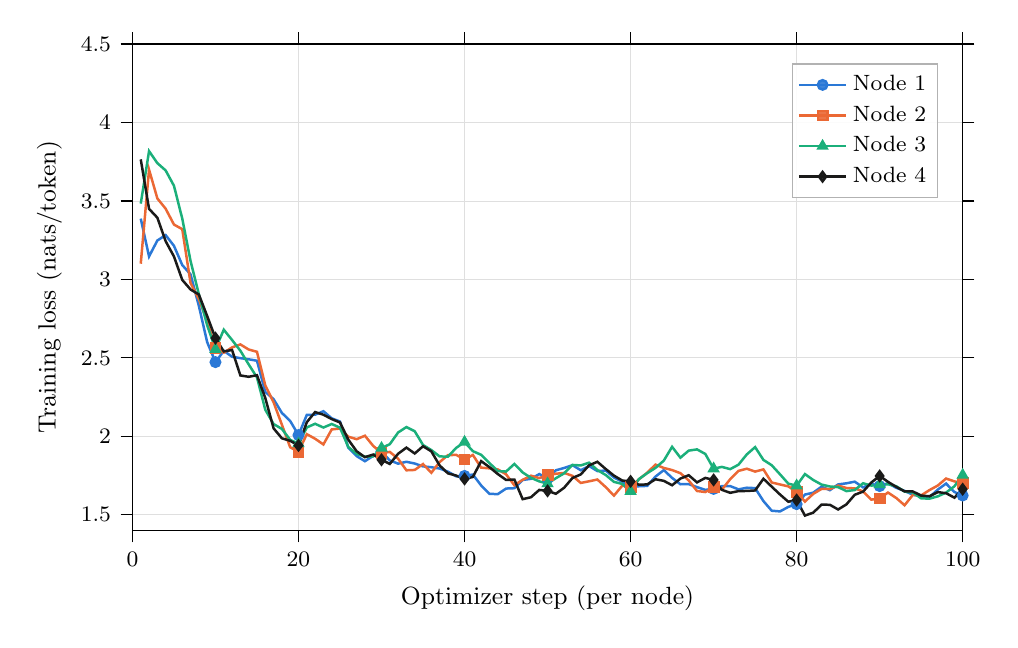
\begin{tikzpicture}
    \begin{axis}[
      width=\linewidth, height=0.64\linewidth,
      xlabel={Optimizer step (per node)},
      ylabel={Training loss (nats/token)},
      xmin=0, xmax=100, ymin=1.4, ymax=4.5,
      xtick={0,20,40,60,80,100},
      ytick={1.5,2.0,2.5,3.0,3.5,4.0,4.5},
      yticklabel style={/pgf/number format/fixed, /pgf/number format/precision=1},
      grid=major, major grid style={gray!25, line width=0.3pt},
      tick align=outside, tick style={black, line width=0.4pt},
      axis line style={black, line width=0.4pt},
      label style={font=\small}, tick label style={font=\footnotesize},
      legend style={at={(0.97,0.96)}, anchor=north east, draw=gray!60, fill=white,
                    fill opacity=0.9, text opacity=1, font=\footnotesize,
                    inner sep=2pt, /tikz/every even column/.append style={column sep=3pt}},
      legend cell align=left,
      every axis plot/.append style={line width=0.9pt, mark size=1.7pt},
    ]
    \addplot[nodeA, mark=*, mark repeat=10, mark phase=10]
      coordinates {(1,3.3874) (2,3.1464) (3,3.2481) (4,3.2825) (5,3.2141) (6,3.0918) (7,3.0323) (8,2.8312) (9,2.6006) (10,2.4731) (11,2.5449) (12,2.5076) (13,2.4983) (14,2.4912) (15,2.4819) (16,2.2834) (17,2.2370) (18,2.1494) (19,2.0980) (20,2.0082) (21,2.1366) (22,2.1382) (23,2.1602) (24,2.1150) (25,2.0943) (26,1.9274) (27,1.8743) (28,1.8417) (29,1.8757) (30,1.9024) (31,1.8468) (32,1.8261) (33,1.8380) (34,1.8270) (35,1.8087) (36,1.8034) (37,1.7951) (38,1.7752) (39,1.7453) (40,1.7481) (41,1.7566) (42,1.6875) (43,1.6338) (44,1.6320) (45,1.6675) (46,1.6697) (47,1.7222) (48,1.7295) (49,1.7596) (50,1.7327) (51,1.7840) (52,1.7986) (53,1.8166) (54,1.7843) (55,1.8112) (56,1.7789) (57,1.7822) (58,1.7378) (59,1.7114) (60,1.6760) (61,1.6821) (62,1.6844) (63,1.7437) (64,1.7851) (65,1.7354) (66,1.6949) (67,1.6958) (68,1.6765) (69,1.6591) (70,1.6652) (71,1.6827) (72,1.6832) (73,1.6622) (74,1.6728) (75,1.6702) (76,1.5877) (77,1.5263) (78,1.5218) (79,1.5506) (80,1.5680) (81,1.6290) (82,1.6413) (83,1.6793) (84,1.6573) (85,1.6939) (86,1.7009) (87,1.7113) (88,1.6749) (89,1.6978) (90,1.6833) (91,1.7020) (92,1.6721) (93,1.6526) (94,1.6281) (95,1.6190) (96,1.6125) (97,1.6607) (98,1.6993) (99,1.6458) (100,1.6232)};
    \addlegendentry{Node 1}
    \addplot[nodeB, mark=square*, mark repeat=10, mark phase=10]
      coordinates {(1,3.1001) (2,3.6995) (3,3.5163) (4,3.4504) (5,3.3496) (6,3.3202) (7,2.9765) (8,2.8741) (9,2.7346) (10,2.5618) (11,2.5331) (12,2.5670) (13,2.5859) (14,2.5535) (15,2.5388) (16,2.3250) (17,2.2170) (18,2.0744) (19,1.9304) (20,1.9026) (21,2.0140) (22,1.9850) (23,1.9485) (24,2.0442) (25,2.0501) (26,1.9982) (27,1.9820) (28,2.0041) (29,1.9392) (30,1.8938) (31,1.9009) (32,1.8574) (33,1.7838) (34,1.7861) (35,1.8237) (36,1.7681) (37,1.8362) (38,1.8804) (39,1.8820) (40,1.8524) (41,1.8817) (42,1.8009) (43,1.7961) (44,1.7898) (45,1.7586) (46,1.6883) (47,1.7232) (48,1.7494) (49,1.7342) (50,1.7533) (51,1.7618) (52,1.7672) (53,1.7485) (54,1.7034) (55,1.7137) (56,1.7251) (57,1.6768) (58,1.6225) (59,1.6861) (60,1.6770) (61,1.7262) (62,1.7685) (63,1.8201) (64,1.7988) (65,1.7853) (66,1.7655) (67,1.7193) (68,1.6520) (69,1.6453) (70,1.6755) (71,1.6603) (72,1.7274) (73,1.7802) (74,1.7939) (75,1.7757) (76,1.7895) (77,1.7061) (78,1.6935) (79,1.6814) (80,1.6476) (81,1.5844) (82,1.6337) (83,1.6651) (84,1.6645) (85,1.6864) (86,1.6711) (87,1.6686) (88,1.6496) (89,1.5970) (90,1.6043) (91,1.6420) (92,1.6073) (93,1.5611) (94,1.6270) (95,1.6240) (96,1.6577) (97,1.6867) (98,1.7313) (99,1.7133) (100,1.7006)};
    \addlegendentry{Node 2}
    \addplot[nodeC, mark=triangle*, mark repeat=10, mark phase=10]
      coordinates {(1,3.4830) (2,3.8176) (3,3.7410) (4,3.6945) (5,3.5968) (6,3.3874) (7,3.1175) (8,2.9054) (9,2.7082) (10,2.5557) (11,2.6797) (12,2.6140) (13,2.5457) (14,2.4587) (15,2.3758) (16,2.1697) (17,2.0786) (18,2.0475) (19,1.9778) (20,1.9540) (21,2.0567) (22,2.0802) (23,2.0563) (24,2.0789) (25,2.0552) (26,1.9323) (27,1.8883) (28,1.8701) (29,1.8722) (30,1.9254) (31,1.9503) (32,2.0248) (33,2.0593) (34,2.0326) (35,1.9452) (36,1.9129) (37,1.8721) (38,1.8711) (39,1.9269) (40,1.9641) (41,1.9059) (42,1.8826) (43,1.8301) (44,1.7790) (45,1.7758) (46,1.8243) (47,1.7702) (48,1.7359) (49,1.7132) (50,1.6990) (51,1.7334) (52,1.7645) (53,1.8180) (54,1.8148) (55,1.8324) (56,1.7855) (57,1.7541) (58,1.7101) (59,1.6970) (60,1.6501) (61,1.7279) (62,1.7654) (63,1.7990) (64,1.8455) (65,1.9334) (66,1.8642) (67,1.9091) (68,1.9171) (69,1.8880) (70,1.7943) (71,1.8055) (72,1.7912) (73,1.8198) (74,1.8853) (75,1.9315) (76,1.8500) (77,1.8161) (78,1.7580) (79,1.6987) (80,1.6859) (81,1.7597) (82,1.7221) (83,1.6929) (84,1.6807) (85,1.6767) (86,1.6512) (87,1.6581) (88,1.7013) (89,1.6862) (90,1.6933) (91,1.6948) (92,1.6822) (93,1.6484) (94,1.6420) (95,1.6051) (96,1.6031) (97,1.6178) (98,1.6419) (99,1.6817) (100,1.7540)};
    \addlegendentry{Node 3}
    \addplot[nodeD, mark=diamond*, mark repeat=10, mark phase=10]
      coordinates {(1,3.7650) (2,3.4496) (3,3.3934) (4,3.2435) (5,3.1462) (6,2.9970) (7,2.9359) (8,2.9038) (9,2.7670) (10,2.6260) (11,2.5413) (12,2.5503) (13,2.3882) (14,2.3797) (15,2.3895) (16,2.2446) (17,2.0513) (18,1.9877) (19,1.9717) (20,1.9423) (21,2.0901) (22,2.1549) (23,2.1381) (24,2.1102) (25,2.0886) (26,1.9789) (27,1.9054) (28,1.8676) (29,1.8842) (30,1.8509) (31,1.8246) (32,1.8893) (33,1.9283) (34,1.8910) (35,1.9370) (36,1.9047) (37,1.8145) (38,1.7643) (39,1.7501) (40,1.7289) (41,1.7414) (42,1.8422) (43,1.8038) (44,1.7603) (45,1.7225) (46,1.7250) (47,1.5999) (48,1.6121) (49,1.6588) (50,1.6528) (51,1.6342) (52,1.6729) (53,1.7348) (54,1.7576) (55,1.8155) (56,1.8381) (57,1.7923) (58,1.7497) (59,1.7186) (60,1.7133) (61,1.6922) (62,1.6939) (63,1.7266) (64,1.7166) (65,1.6887) (66,1.7310) (67,1.7525) (68,1.7069) (69,1.7353) (70,1.7227) (71,1.6592) (72,1.6403) (73,1.6512) (74,1.6521) (75,1.6554) (76,1.7300) (77,1.6795) (78,1.6295) (79,1.5834) (80,1.5940) (81,1.4954) (82,1.5139) (83,1.5649) (84,1.5641) (85,1.5342) (86,1.5668) (87,1.6279) (88,1.6479) (89,1.7063) (90,1.7479) (91,1.7105) (92,1.6780) (93,1.6498) (94,1.6490) (95,1.6227) (96,1.6183) (97,1.6449) (98,1.6379) (99,1.6095) (100,1.6633)};
    \addlegendentry{Node 4}
    \end{axis}
  \end{tikzpicture}
  \caption{Training loss of the four federated nodes during LoRA fine-tuning of OLMo-2~1B on the
  South Asia corpus. The loss is the token-weighted negative log-likelihood of the assistant-response
  tokens at each optimizer step (16 packed sequences of 2{,}048 tokens), smoothed with a trailing
  5-step moving average. Each federated round consists of 10 local steps followed by trust-weighted
  aggregation of the sparsified LoRA updates; markers indicate round boundaries. All nodes use identical
  hyper-parameters (AdamW, peak learning rate $2\times10^{-4}$, a single cosine schedule over 100 steps)
  and disjoint data shards.}
  \label{fig:sft-train-loss}
\end{figure}
 where the figure should appear.
% (Colours are colour-blind-safe and every node also has its own marker.)
\begin{figure}[t]
  \centering
  \definecolor{nodeA}{HTML}{2A78D6}
  \definecolor{nodeB}{HTML}{EB6834}
  \definecolor{nodeC}{HTML}{1BAF7A}
  \definecolor{nodeD}{HTML}{1A1A19}
  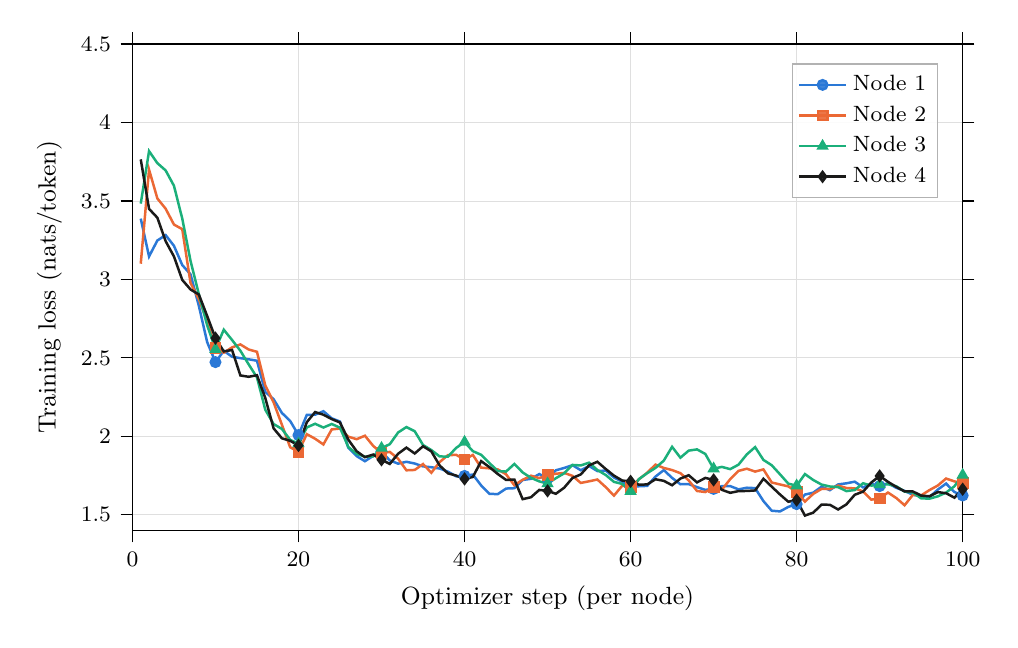
\begin{tikzpicture}
    \begin{axis}[
      width=\linewidth, height=0.64\linewidth,
      xlabel={Optimizer step (per node)},
      ylabel={Training loss (nats/token)},
      xmin=0, xmax=100, ymin=1.4, ymax=4.5,
      xtick={0,20,40,60,80,100},
      ytick={1.5,2.0,2.5,3.0,3.5,4.0,4.5},
      yticklabel style={/pgf/number format/fixed, /pgf/number format/precision=1},
      grid=major, major grid style={gray!25, line width=0.3pt},
      tick align=outside, tick style={black, line width=0.4pt},
      axis line style={black, line width=0.4pt},
      label style={font=\small}, tick label style={font=\footnotesize},
      legend style={at={(0.97,0.96)}, anchor=north east, draw=gray!60, fill=white,
                    fill opacity=0.9, text opacity=1, font=\footnotesize,
                    inner sep=2pt, /tikz/every even column/.append style={column sep=3pt}},
      legend cell align=left,
      every axis plot/.append style={line width=0.9pt, mark size=1.7pt},
    ]
    \addplot[nodeA, mark=*, mark repeat=10, mark phase=10]
      coordinates {(1,3.3874) (2,3.1464) (3,3.2481) (4,3.2825) (5,3.2141) (6,3.0918) (7,3.0323) (8,2.8312) (9,2.6006) (10,2.4731) (11,2.5449) (12,2.5076) (13,2.4983) (14,2.4912) (15,2.4819) (16,2.2834) (17,2.2370) (18,2.1494) (19,2.0980) (20,2.0082) (21,2.1366) (22,2.1382) (23,2.1602) (24,2.1150) (25,2.0943) (26,1.9274) (27,1.8743) (28,1.8417) (29,1.8757) (30,1.9024) (31,1.8468) (32,1.8261) (33,1.8380) (34,1.8270) (35,1.8087) (36,1.8034) (37,1.7951) (38,1.7752) (39,1.7453) (40,1.7481) (41,1.7566) (42,1.6875) (43,1.6338) (44,1.6320) (45,1.6675) (46,1.6697) (47,1.7222) (48,1.7295) (49,1.7596) (50,1.7327) (51,1.7840) (52,1.7986) (53,1.8166) (54,1.7843) (55,1.8112) (56,1.7789) (57,1.7822) (58,1.7378) (59,1.7114) (60,1.6760) (61,1.6821) (62,1.6844) (63,1.7437) (64,1.7851) (65,1.7354) (66,1.6949) (67,1.6958) (68,1.6765) (69,1.6591) (70,1.6652) (71,1.6827) (72,1.6832) (73,1.6622) (74,1.6728) (75,1.6702) (76,1.5877) (77,1.5263) (78,1.5218) (79,1.5506) (80,1.5680) (81,1.6290) (82,1.6413) (83,1.6793) (84,1.6573) (85,1.6939) (86,1.7009) (87,1.7113) (88,1.6749) (89,1.6978) (90,1.6833) (91,1.7020) (92,1.6721) (93,1.6526) (94,1.6281) (95,1.6190) (96,1.6125) (97,1.6607) (98,1.6993) (99,1.6458) (100,1.6232)};
    \addlegendentry{Node 1}
    \addplot[nodeB, mark=square*, mark repeat=10, mark phase=10]
      coordinates {(1,3.1001) (2,3.6995) (3,3.5163) (4,3.4504) (5,3.3496) (6,3.3202) (7,2.9765) (8,2.8741) (9,2.7346) (10,2.5618) (11,2.5331) (12,2.5670) (13,2.5859) (14,2.5535) (15,2.5388) (16,2.3250) (17,2.2170) (18,2.0744) (19,1.9304) (20,1.9026) (21,2.0140) (22,1.9850) (23,1.9485) (24,2.0442) (25,2.0501) (26,1.9982) (27,1.9820) (28,2.0041) (29,1.9392) (30,1.8938) (31,1.9009) (32,1.8574) (33,1.7838) (34,1.7861) (35,1.8237) (36,1.7681) (37,1.8362) (38,1.8804) (39,1.8820) (40,1.8524) (41,1.8817) (42,1.8009) (43,1.7961) (44,1.7898) (45,1.7586) (46,1.6883) (47,1.7232) (48,1.7494) (49,1.7342) (50,1.7533) (51,1.7618) (52,1.7672) (53,1.7485) (54,1.7034) (55,1.7137) (56,1.7251) (57,1.6768) (58,1.6225) (59,1.6861) (60,1.6770) (61,1.7262) (62,1.7685) (63,1.8201) (64,1.7988) (65,1.7853) (66,1.7655) (67,1.7193) (68,1.6520) (69,1.6453) (70,1.6755) (71,1.6603) (72,1.7274) (73,1.7802) (74,1.7939) (75,1.7757) (76,1.7895) (77,1.7061) (78,1.6935) (79,1.6814) (80,1.6476) (81,1.5844) (82,1.6337) (83,1.6651) (84,1.6645) (85,1.6864) (86,1.6711) (87,1.6686) (88,1.6496) (89,1.5970) (90,1.6043) (91,1.6420) (92,1.6073) (93,1.5611) (94,1.6270) (95,1.6240) (96,1.6577) (97,1.6867) (98,1.7313) (99,1.7133) (100,1.7006)};
    \addlegendentry{Node 2}
    \addplot[nodeC, mark=triangle*, mark repeat=10, mark phase=10]
      coordinates {(1,3.4830) (2,3.8176) (3,3.7410) (4,3.6945) (5,3.5968) (6,3.3874) (7,3.1175) (8,2.9054) (9,2.7082) (10,2.5557) (11,2.6797) (12,2.6140) (13,2.5457) (14,2.4587) (15,2.3758) (16,2.1697) (17,2.0786) (18,2.0475) (19,1.9778) (20,1.9540) (21,2.0567) (22,2.0802) (23,2.0563) (24,2.0789) (25,2.0552) (26,1.9323) (27,1.8883) (28,1.8701) (29,1.8722) (30,1.9254) (31,1.9503) (32,2.0248) (33,2.0593) (34,2.0326) (35,1.9452) (36,1.9129) (37,1.8721) (38,1.8711) (39,1.9269) (40,1.9641) (41,1.9059) (42,1.8826) (43,1.8301) (44,1.7790) (45,1.7758) (46,1.8243) (47,1.7702) (48,1.7359) (49,1.7132) (50,1.6990) (51,1.7334) (52,1.7645) (53,1.8180) (54,1.8148) (55,1.8324) (56,1.7855) (57,1.7541) (58,1.7101) (59,1.6970) (60,1.6501) (61,1.7279) (62,1.7654) (63,1.7990) (64,1.8455) (65,1.9334) (66,1.8642) (67,1.9091) (68,1.9171) (69,1.8880) (70,1.7943) (71,1.8055) (72,1.7912) (73,1.8198) (74,1.8853) (75,1.9315) (76,1.8500) (77,1.8161) (78,1.7580) (79,1.6987) (80,1.6859) (81,1.7597) (82,1.7221) (83,1.6929) (84,1.6807) (85,1.6767) (86,1.6512) (87,1.6581) (88,1.7013) (89,1.6862) (90,1.6933) (91,1.6948) (92,1.6822) (93,1.6484) (94,1.6420) (95,1.6051) (96,1.6031) (97,1.6178) (98,1.6419) (99,1.6817) (100,1.7540)};
    \addlegendentry{Node 3}
    \addplot[nodeD, mark=diamond*, mark repeat=10, mark phase=10]
      coordinates {(1,3.7650) (2,3.4496) (3,3.3934) (4,3.2435) (5,3.1462) (6,2.9970) (7,2.9359) (8,2.9038) (9,2.7670) (10,2.6260) (11,2.5413) (12,2.5503) (13,2.3882) (14,2.3797) (15,2.3895) (16,2.2446) (17,2.0513) (18,1.9877) (19,1.9717) (20,1.9423) (21,2.0901) (22,2.1549) (23,2.1381) (24,2.1102) (25,2.0886) (26,1.9789) (27,1.9054) (28,1.8676) (29,1.8842) (30,1.8509) (31,1.8246) (32,1.8893) (33,1.9283) (34,1.8910) (35,1.9370) (36,1.9047) (37,1.8145) (38,1.7643) (39,1.7501) (40,1.7289) (41,1.7414) (42,1.8422) (43,1.8038) (44,1.7603) (45,1.7225) (46,1.7250) (47,1.5999) (48,1.6121) (49,1.6588) (50,1.6528) (51,1.6342) (52,1.6729) (53,1.7348) (54,1.7576) (55,1.8155) (56,1.8381) (57,1.7923) (58,1.7497) (59,1.7186) (60,1.7133) (61,1.6922) (62,1.6939) (63,1.7266) (64,1.7166) (65,1.6887) (66,1.7310) (67,1.7525) (68,1.7069) (69,1.7353) (70,1.7227) (71,1.6592) (72,1.6403) (73,1.6512) (74,1.6521) (75,1.6554) (76,1.7300) (77,1.6795) (78,1.6295) (79,1.5834) (80,1.5940) (81,1.4954) (82,1.5139) (83,1.5649) (84,1.5641) (85,1.5342) (86,1.5668) (87,1.6279) (88,1.6479) (89,1.7063) (90,1.7479) (91,1.7105) (92,1.6780) (93,1.6498) (94,1.6490) (95,1.6227) (96,1.6183) (97,1.6449) (98,1.6379) (99,1.6095) (100,1.6633)};
    \addlegendentry{Node 4}
    \end{axis}
  \end{tikzpicture}
  \caption{Training loss of the four federated nodes during LoRA fine-tuning of OLMo-2~1B on the
  South Asia corpus. The loss is the token-weighted negative log-likelihood of the assistant-response
  tokens at each optimizer step (16 packed sequences of 2{,}048 tokens), smoothed with a trailing
  5-step moving average. Each federated round consists of 10 local steps followed by trust-weighted
  aggregation of the sparsified LoRA updates; markers indicate round boundaries. All nodes use identical
  hyper-parameters (AdamW, peak learning rate $2\times10^{-4}$, a single cosine schedule over 100 steps)
  and disjoint data shards.}
  \label{fig:sft-train-loss}
\end{figure}
 where the figure should appear.
% (Colours are colour-blind-safe and every node also has its own marker.)
\begin{figure}[t]
  \centering
  \definecolor{nodeA}{HTML}{2A78D6}
  \definecolor{nodeB}{HTML}{EB6834}
  \definecolor{nodeC}{HTML}{1BAF7A}
  \definecolor{nodeD}{HTML}{1A1A19}
  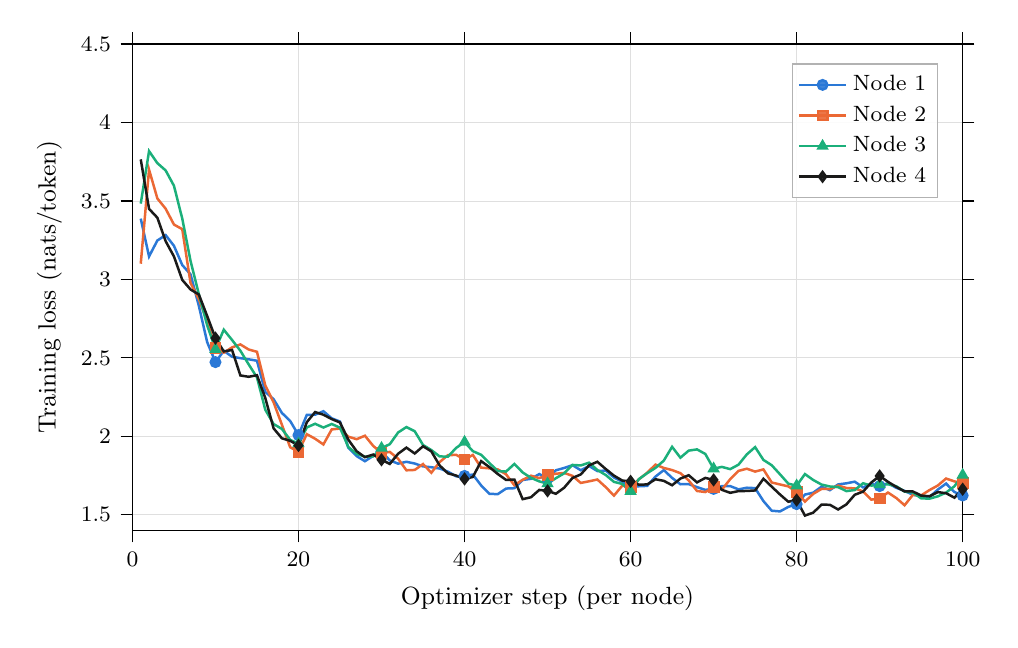
\begin{tikzpicture}
    \begin{axis}[
      width=\linewidth, height=0.64\linewidth,
      xlabel={Optimizer step (per node)},
      ylabel={Training loss (nats/token)},
      xmin=0, xmax=100, ymin=1.4, ymax=4.5,
      xtick={0,20,40,60,80,100},
      ytick={1.5,2.0,2.5,3.0,3.5,4.0,4.5},
      yticklabel style={/pgf/number format/fixed, /pgf/number format/precision=1},
      grid=major, major grid style={gray!25, line width=0.3pt},
      tick align=outside, tick style={black, line width=0.4pt},
      axis line style={black, line width=0.4pt},
      label style={font=\small}, tick label style={font=\footnotesize},
      legend style={at={(0.97,0.96)}, anchor=north east, draw=gray!60, fill=white,
                    fill opacity=0.9, text opacity=1, font=\footnotesize,
                    inner sep=2pt, /tikz/every even column/.append style={column sep=3pt}},
      legend cell align=left,
      every axis plot/.append style={line width=0.9pt, mark size=1.7pt},
    ]
    \addplot[nodeA, mark=*, mark repeat=10, mark phase=10]
      coordinates {(1,3.3874) (2,3.1464) (3,3.2481) (4,3.2825) (5,3.2141) (6,3.0918) (7,3.0323) (8,2.8312) (9,2.6006) (10,2.4731) (11,2.5449) (12,2.5076) (13,2.4983) (14,2.4912) (15,2.4819) (16,2.2834) (17,2.2370) (18,2.1494) (19,2.0980) (20,2.0082) (21,2.1366) (22,2.1382) (23,2.1602) (24,2.1150) (25,2.0943) (26,1.9274) (27,1.8743) (28,1.8417) (29,1.8757) (30,1.9024) (31,1.8468) (32,1.8261) (33,1.8380) (34,1.8270) (35,1.8087) (36,1.8034) (37,1.7951) (38,1.7752) (39,1.7453) (40,1.7481) (41,1.7566) (42,1.6875) (43,1.6338) (44,1.6320) (45,1.6675) (46,1.6697) (47,1.7222) (48,1.7295) (49,1.7596) (50,1.7327) (51,1.7840) (52,1.7986) (53,1.8166) (54,1.7843) (55,1.8112) (56,1.7789) (57,1.7822) (58,1.7378) (59,1.7114) (60,1.6760) (61,1.6821) (62,1.6844) (63,1.7437) (64,1.7851) (65,1.7354) (66,1.6949) (67,1.6958) (68,1.6765) (69,1.6591) (70,1.6652) (71,1.6827) (72,1.6832) (73,1.6622) (74,1.6728) (75,1.6702) (76,1.5877) (77,1.5263) (78,1.5218) (79,1.5506) (80,1.5680) (81,1.6290) (82,1.6413) (83,1.6793) (84,1.6573) (85,1.6939) (86,1.7009) (87,1.7113) (88,1.6749) (89,1.6978) (90,1.6833) (91,1.7020) (92,1.6721) (93,1.6526) (94,1.6281) (95,1.6190) (96,1.6125) (97,1.6607) (98,1.6993) (99,1.6458) (100,1.6232)};
    \addlegendentry{Node 1}
    \addplot[nodeB, mark=square*, mark repeat=10, mark phase=10]
      coordinates {(1,3.1001) (2,3.6995) (3,3.5163) (4,3.4504) (5,3.3496) (6,3.3202) (7,2.9765) (8,2.8741) (9,2.7346) (10,2.5618) (11,2.5331) (12,2.5670) (13,2.5859) (14,2.5535) (15,2.5388) (16,2.3250) (17,2.2170) (18,2.0744) (19,1.9304) (20,1.9026) (21,2.0140) (22,1.9850) (23,1.9485) (24,2.0442) (25,2.0501) (26,1.9982) (27,1.9820) (28,2.0041) (29,1.9392) (30,1.8938) (31,1.9009) (32,1.8574) (33,1.7838) (34,1.7861) (35,1.8237) (36,1.7681) (37,1.8362) (38,1.8804) (39,1.8820) (40,1.8524) (41,1.8817) (42,1.8009) (43,1.7961) (44,1.7898) (45,1.7586) (46,1.6883) (47,1.7232) (48,1.7494) (49,1.7342) (50,1.7533) (51,1.7618) (52,1.7672) (53,1.7485) (54,1.7034) (55,1.7137) (56,1.7251) (57,1.6768) (58,1.6225) (59,1.6861) (60,1.6770) (61,1.7262) (62,1.7685) (63,1.8201) (64,1.7988) (65,1.7853) (66,1.7655) (67,1.7193) (68,1.6520) (69,1.6453) (70,1.6755) (71,1.6603) (72,1.7274) (73,1.7802) (74,1.7939) (75,1.7757) (76,1.7895) (77,1.7061) (78,1.6935) (79,1.6814) (80,1.6476) (81,1.5844) (82,1.6337) (83,1.6651) (84,1.6645) (85,1.6864) (86,1.6711) (87,1.6686) (88,1.6496) (89,1.5970) (90,1.6043) (91,1.6420) (92,1.6073) (93,1.5611) (94,1.6270) (95,1.6240) (96,1.6577) (97,1.6867) (98,1.7313) (99,1.7133) (100,1.7006)};
    \addlegendentry{Node 2}
    \addplot[nodeC, mark=triangle*, mark repeat=10, mark phase=10]
      coordinates {(1,3.4830) (2,3.8176) (3,3.7410) (4,3.6945) (5,3.5968) (6,3.3874) (7,3.1175) (8,2.9054) (9,2.7082) (10,2.5557) (11,2.6797) (12,2.6140) (13,2.5457) (14,2.4587) (15,2.3758) (16,2.1697) (17,2.0786) (18,2.0475) (19,1.9778) (20,1.9540) (21,2.0567) (22,2.0802) (23,2.0563) (24,2.0789) (25,2.0552) (26,1.9323) (27,1.8883) (28,1.8701) (29,1.8722) (30,1.9254) (31,1.9503) (32,2.0248) (33,2.0593) (34,2.0326) (35,1.9452) (36,1.9129) (37,1.8721) (38,1.8711) (39,1.9269) (40,1.9641) (41,1.9059) (42,1.8826) (43,1.8301) (44,1.7790) (45,1.7758) (46,1.8243) (47,1.7702) (48,1.7359) (49,1.7132) (50,1.6990) (51,1.7334) (52,1.7645) (53,1.8180) (54,1.8148) (55,1.8324) (56,1.7855) (57,1.7541) (58,1.7101) (59,1.6970) (60,1.6501) (61,1.7279) (62,1.7654) (63,1.7990) (64,1.8455) (65,1.9334) (66,1.8642) (67,1.9091) (68,1.9171) (69,1.8880) (70,1.7943) (71,1.8055) (72,1.7912) (73,1.8198) (74,1.8853) (75,1.9315) (76,1.8500) (77,1.8161) (78,1.7580) (79,1.6987) (80,1.6859) (81,1.7597) (82,1.7221) (83,1.6929) (84,1.6807) (85,1.6767) (86,1.6512) (87,1.6581) (88,1.7013) (89,1.6862) (90,1.6933) (91,1.6948) (92,1.6822) (93,1.6484) (94,1.6420) (95,1.6051) (96,1.6031) (97,1.6178) (98,1.6419) (99,1.6817) (100,1.7540)};
    \addlegendentry{Node 3}
    \addplot[nodeD, mark=diamond*, mark repeat=10, mark phase=10]
      coordinates {(1,3.7650) (2,3.4496) (3,3.3934) (4,3.2435) (5,3.1462) (6,2.9970) (7,2.9359) (8,2.9038) (9,2.7670) (10,2.6260) (11,2.5413) (12,2.5503) (13,2.3882) (14,2.3797) (15,2.3895) (16,2.2446) (17,2.0513) (18,1.9877) (19,1.9717) (20,1.9423) (21,2.0901) (22,2.1549) (23,2.1381) (24,2.1102) (25,2.0886) (26,1.9789) (27,1.9054) (28,1.8676) (29,1.8842) (30,1.8509) (31,1.8246) (32,1.8893) (33,1.9283) (34,1.8910) (35,1.9370) (36,1.9047) (37,1.8145) (38,1.7643) (39,1.7501) (40,1.7289) (41,1.7414) (42,1.8422) (43,1.8038) (44,1.7603) (45,1.7225) (46,1.7250) (47,1.5999) (48,1.6121) (49,1.6588) (50,1.6528) (51,1.6342) (52,1.6729) (53,1.7348) (54,1.7576) (55,1.8155) (56,1.8381) (57,1.7923) (58,1.7497) (59,1.7186) (60,1.7133) (61,1.6922) (62,1.6939) (63,1.7266) (64,1.7166) (65,1.6887) (66,1.7310) (67,1.7525) (68,1.7069) (69,1.7353) (70,1.7227) (71,1.6592) (72,1.6403) (73,1.6512) (74,1.6521) (75,1.6554) (76,1.7300) (77,1.6795) (78,1.6295) (79,1.5834) (80,1.5940) (81,1.4954) (82,1.5139) (83,1.5649) (84,1.5641) (85,1.5342) (86,1.5668) (87,1.6279) (88,1.6479) (89,1.7063) (90,1.7479) (91,1.7105) (92,1.6780) (93,1.6498) (94,1.6490) (95,1.6227) (96,1.6183) (97,1.6449) (98,1.6379) (99,1.6095) (100,1.6633)};
    \addlegendentry{Node 4}
    \end{axis}
  \end{tikzpicture}
  \caption{Training loss of the four federated nodes during LoRA fine-tuning of OLMo-2~1B on the
  South Asia corpus. The loss is the token-weighted negative log-likelihood of the assistant-response
  tokens at each optimizer step (16 packed sequences of 2{,}048 tokens), smoothed with a trailing
  5-step moving average. Each federated round consists of 10 local steps followed by trust-weighted
  aggregation of the sparsified LoRA updates; markers indicate round boundaries. All nodes use identical
  hyper-parameters (AdamW, peak learning rate $2\times10^{-4}$, a single cosine schedule over 100 steps)
  and disjoint data shards.}
  \label{fig:sft-train-loss}
\end{figure}
